\chapter{Experiments}
\label{sec:experiments}

This study investigates the capabilities and limitations of restricted Boltzmann machines
for the classical simulation of quantum computing. For this purpose, the approach of Janson 
et al. \cite{jnsson2018neuralnetwork} has been adapted to simulate random circuit instances \cite{Boixo2018supremacy}.
These kinds of experiments have recently been conducted on a 53 superconducting qubit quantum computer \cite{martines2019supremacy}.

\section{Setup}
\label{sec:setup}

In order to run the experiments, Netket, an open-source library for the classical simulation of quantum 
many-body systems \cite{netket2019}, has been extended to simulate quantum circuits given in the QASM format \cite{cross2017open}. The resulting 
software is published at \cite{} as an open-source tool for the classical simulation 
of quantum circuits. The experiments have been conducted on the Noctua Cluster at the University of Paderborn, Germany.

Several parameters of the RBM's training process have been varied. For the choice of the optimization algorithm, AdaMax and 
Stochastic Reconfiguration are tested against each other. Performances of different numbers of training iterations 
as well as training samples are compared. Further, the controlled-Z ($CZ$) gate is applied in two fashions: Once, 
by following the rules from \cite{jnsson2018neuralnetwork} by introducing an additional hidden unit to the RBM on each gate. In other 
experiments, the CZ gate is applied by training the parameters of the RBM the same way as for 
non-diagonal gates. In the first case, the RBM is initialized without any hidden units. In the latter 
case, it is initialized with so many hidden units that each pair of visible units is connected 
by one hidden unit. This corresponds to 6 hidden units for RBMs with 4 visible units.

The training process is once performed with \textit{random restarts} and once without. 
In the experiments with random restarts, the RBM is trained several times with a slight Gaussian noise modification to its 
current parameters and the best performing resulting parameters are chosen as the after gate parameters. 

The gate set of the circuits consists of the $T$, $\sqrt{X}$, $\sqrt{Y}$, and $CZ$ gate. While the $CZ$ gate is 
applied in different manners as described above, the $T$ gate is a diagonal gate and can be applied exactly to the RBM state.
The $\sqrt{X}$ and $\sqrt{Y}$ gates are non-diagonal and are thus applied by adopting the parameters of the RBM in 
a training phase. The training samples have been chosen $i.i.d$ uniformly at random. 
With a high probability $n, n^2, n^3, 2^n, 0.95 \times 2^n, 0.9 \times 2^n$ and $0.85 \times 2^n$,
respectively, different samples are included in the training set. In the case of 4 qubits, this corresponds to 
8, 43, 47, 50, 54, and 303 samples. The training was performed on batches of the samples with 
up to 10 samples per batch.
The number of training iterations has been chosen as 1,000, 10,000, and 100,000. 

For each parameter setting, five RBMs have been trained on 20 different instances of random circuits of the same 
size. The total variation distance (TVD) as well as the cross entropy fidelity have been used as a performance measure.
The total variation distance measures the sum of absolute differences of two probability distributions. 
It is a more direct measure than the cross entropy fidelity as later is an upper bound on the TVD \cite{bouland2018quantum}.
The training parameters have first been tested on random circuit instances with 4 qubits and 
5, 10, 15, and 20 cycles each. 

The resulting experiments are \textit{AdaMax-restarts-learned}, \textit{SR-restarts-learned}, 
\textit{SR-restarts-not-learned} and \textit{SR-no-restarts-learned}. 

The study compares three different setups for SR with one setup for RBMs trained with 
AdaMax. The reason to vary the parameters for SR but not for AdaMax is twofold:
First, limited access to the cluster did not allow to test all possible parameter combinations. Second,
pre-studies, conducted as part of this study, suggested that AdaMax without random restarts 
was inferior to SR concerning the TVD between the RBMs state and the true output distribution of the 
circuits tested. RBMs trained with AdaMax in those settings repeatedly could not reduce the 
log overlap below a certain threshold during the training.

\section{Results}
\label{sec:results}

In total, 33,600 classical simulations of random quantum circuits have been performed 
on the Noctua cluster over 8 weeks. In each run, the total variation distance (TVD)
between the RBM's output probability and the true output probabilities have been measured.
 The log overlaps of the RBM's state and the distribution on the training and test sets have been recorded during the training process. This allows for a detailed comparison
of the different training methods and the influence of the different training parameters on the 
accuracy of the RBM. Further, the cross entropy fidelity on the circuits' mean outcome probabilities
has been calculated. The following four sections present the results of the 4 training setups.

\subsection{Stochastic Reconfiguration with Random Restarts and CZ-Gates Learned}

Stochastic Reconfiguration (SR) has been successfully used to train RBMs to represent the wave function 
of many-body quantum systems before \cite{}. In this study, SR has been applied with random restarts 
and without. 
This section summarizes the results of RBMs that have been trained with the SR optimizer and five random 
restarts.

Figure~\ref{fig:sr_restarts_avgPDF} shows the averaged output distribution of all RBMs and 
the averaged true output distributions of all circuits. With an increasing number of cycles, the 
true output distributions approach a Porter-Thomas shape, even though they are not exactly Porter-Thomas 
distributed.
The TVD of the average output of all RBMs considered 
is 0.30 for 5, 0.34 for 10, 0.34 for 15, and 0.35 for 20 cycles. The corresponding cross entropy is 
0.16 for 5, 0.05 for 10, 0.04 for 15, and 0.00 for 20 cycles.

\begin{figure}[H]
  \centering
  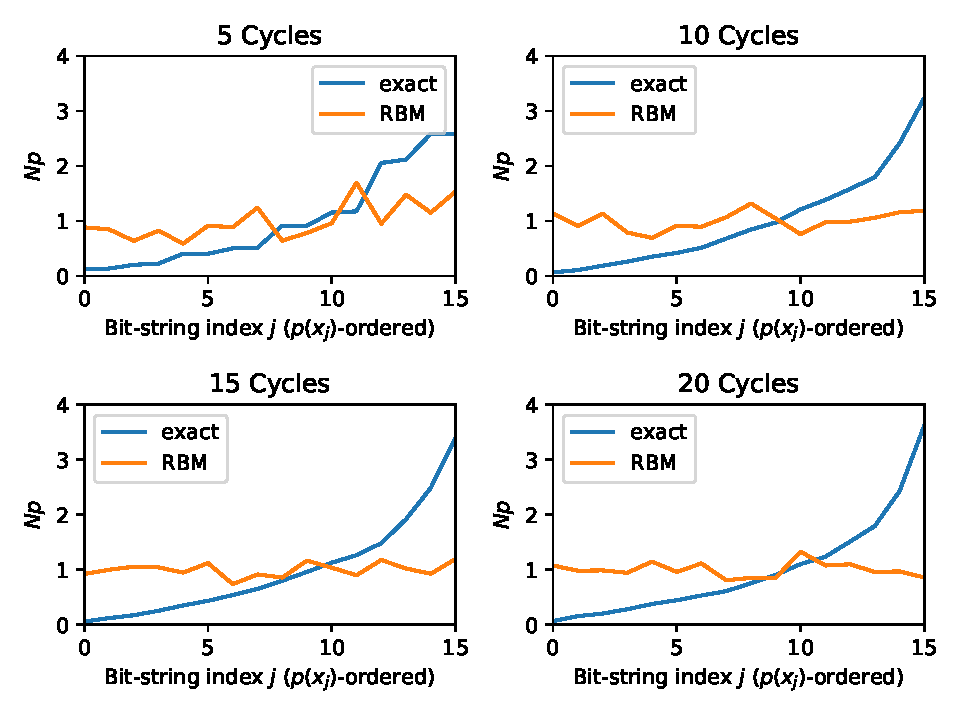
\includegraphics[width=\textwidth]{figures/results/SR-restarts-learned/avgPDF.pdf}
  \caption[Scaled average output probabilities of Stochastic Reconfiguration with Restarts Learned]{
    Scaled average output probabilities of Stochastic Reconfiguration with Restarts and the $CZ$ gates learned. The true 
    output distribution approaches a Porter-Thomas shape with increasing number of cycles.}
  \label{fig:sr_restarts_avgPDF}
\end{figure}

In figure~\ref{fig:sr_restarts_bestPDF}, only the output distribution of the best performing RBMs with respect to the 
TVD are selected and their outputs are averaged. The averaged best output distribution for the SR methods with 
random restarts and $CZ$ gates learned has a TVD of 0.06 for 5, 0.15 for 10, 0.19 for 15, and 0.24 for 20
cycles. The cross entropy fidelity is 0.65 for 5, 0.47 for 10, 0.39 for 15, and 0.31 for 20 cycles each. 

\begin{figure}[H]
  \centering
  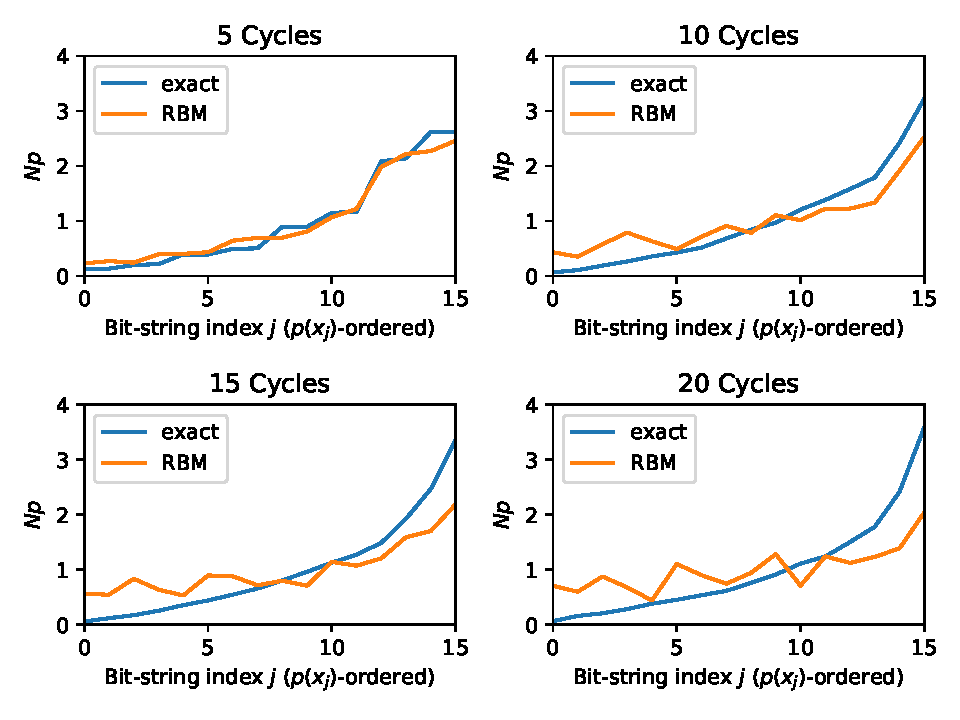
\includegraphics[width=\textwidth]{figures/results/SR-restarts-learned/avgBestPDF.pdf}
  \caption[Averaged best performing scaled output probabilities of Stochastic Reconfiguration with Restarts Learned]{
    Scaled average output probabilities of Stochastic Reconfiguration with Restarts and the $CZ$ gate learned, only RBMs with lowest
    TVD for each circuit are considered.}
  \label{fig:sr_restarts_bestPDF}
\end{figure}

Figure~\ref{fig:sr_restarts_tvd} and figure~\ref{fig:sr_restarts_fxeb} give a more detailed overview of the influence of the 
number of training samples and training iterations on the TVD and cross entropy fidelity. 

There is no correlation between the number of training
iterations and the performance of the RBMs. For 5 cycles, a higher number of training samples correlates
with a lower TVD, independent of the number of training iterations. The RBMs perform best on 
circuits with a depth of 5 cycles when trained with 100,000 iterations and 303 samples. In that case, 
it achieves a mean TVD of $0.50$. The mean TVD is similar when trained with 303 samples and 1,000 iterations, 
where it is $0.51$. When trained with fewer samples, the TVD is generally lowest when trained with 1,000 
iterations and highest when trained with 10,000 iterations for all number of samples tested. 

For 10 cycles, RBMs trained for 1,000 training iterations achieve the lowest TVDs in the range of 43 to 
54 samples. For 303 samples, 100,000 iterations lead to the lowest TVD (0.59). Except for the 
case of 47 samples, 10,000 iterations correlate with the highest TVD.

For 15 and 20 cycles, again, 10,000 training iterations correlate with the lowest TVD in most cases. 1,000
and 100,000 iterations perform similar, with the lowest TVDs on these circuits being achieved with 50 samples and 
100,000 iterations on 15 cycles ($0.62$), and 47 samples with 100,000 iterations on 20 cycles (TVD of $0.68$).

\begin{figure}[H]
  \centering
  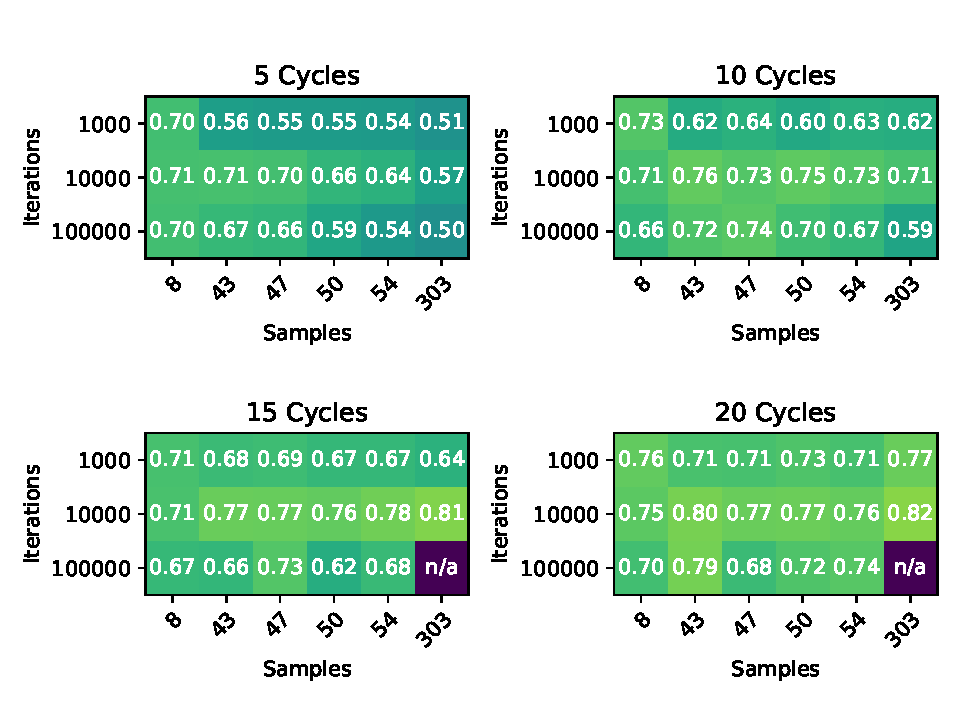
\includegraphics[width=\textwidth]{figures/results/SR-restarts-learned/tvd_heatmap.pdf}
  \caption[TVD of Stochastic Reconfiguration with Restarts Learned]{TVD of Stochastic 
  Reconfiguration with Restarts Learned for the combinations of iterations and samples tested.
  For 100,000 iterations and 303 samples, the experiments did not finish within the time limit.}
  \label{fig:sr_restarts_tvd}
\end{figure}

A lower TVD does not always correlate with a higher cross entropy fidelity as figure~\ref{fig:sr_restarts_fxeb}
shows. On 5 cycles, the highest fidelity is achieved with 303 samples and 10,000 iterations, on 10 cycles 
with 303 samples and 100,000 iterations. On 15 cycles, 8 samples and 1,000 iterations led to the best performance, 
and 47 samples with 100,000 iterations on 20 cycles. Overall, there is a tendency for a higher cross entropy fidelity 
when trained with more samples for 5 and 10 cycles. For 15 cycles, there is no clear correlation between the 
cross entropy fidelity and the training parameters. For circuits with 20 cycles, 47 samples achieved the highest 
fidelity for all number of training samples.

\begin{figure}[H]
  \centering
  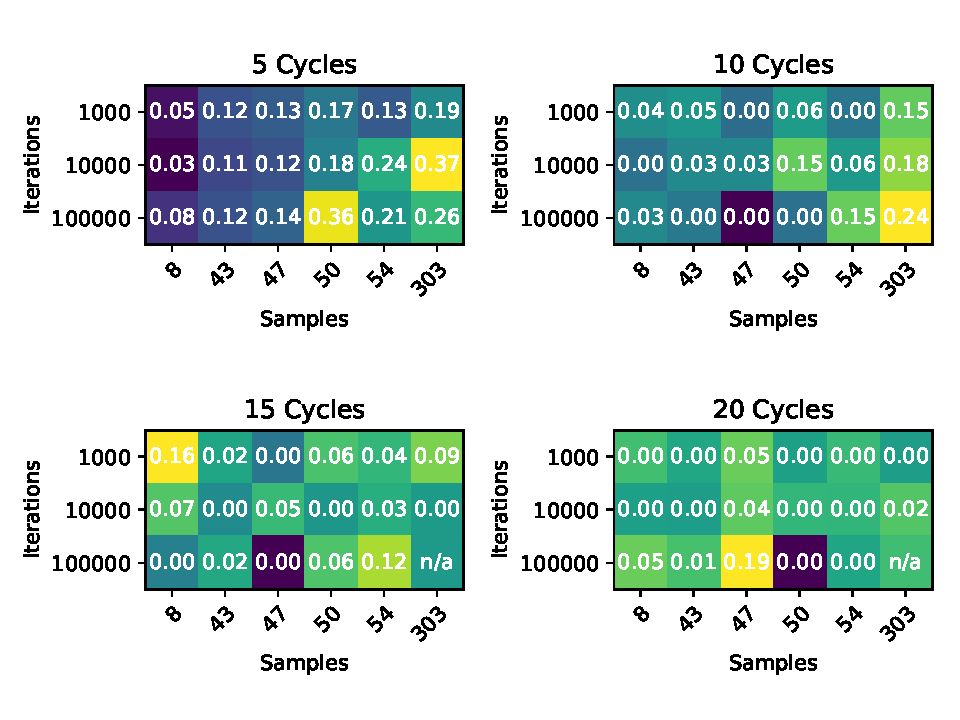
\includegraphics[width=\textwidth]{figures/results/SR-restarts-learned/fxeb_heatmap.pdf}
  \caption[Cross-entropy Fidelity of Stochastic Reconfiguration with Restarts Learned]{Cross-entropy Fidelity of Stochastic 
  Reconfiguration with Restarts and the $CZ$ gates learned for the combinations of iterations and samples tested.}
  \label{fig:sr_restarts_fxeb}
\end{figure}

Figure~\ref{fig:sr_restarts_overlap_8} to~\ref{fig:sr_restarts_overlap_303} details the mean log overlap of the RBMs during the 
training process when trained with 10,000 iterations for 8, 47, and 303 samples. The 
mean overlap of the RBM's state and the distribution implied by the training and test data sets are measured 
for each training iteration.

For 8 samples, the log overlap on the training set can be reduced to almost 0 within the first few training iterations 
on all three gates. For the $\sqrt{Y}$ gate there is a second small dip after about 2,500 training iterations. 
The log overlap on the test set stays slightly below $0.60$ for the single-qubit gates and at about $0.80$ for the 
$CZ$ gate. 

During the whole process and averaged over all three gates, the log overlap is slightly above $0$ in the training data. There is a small 
improvement within the first few training iterations and another small improvement at around 2,500 training iterations. 
The overall log overlap in the test data is about $0.6$ and does not change much during the training process. It 
slightly increases within the first few iterations and goes down a little bit again at about 2,500 training iterations.

\begin{figure}[H]
  \centering
  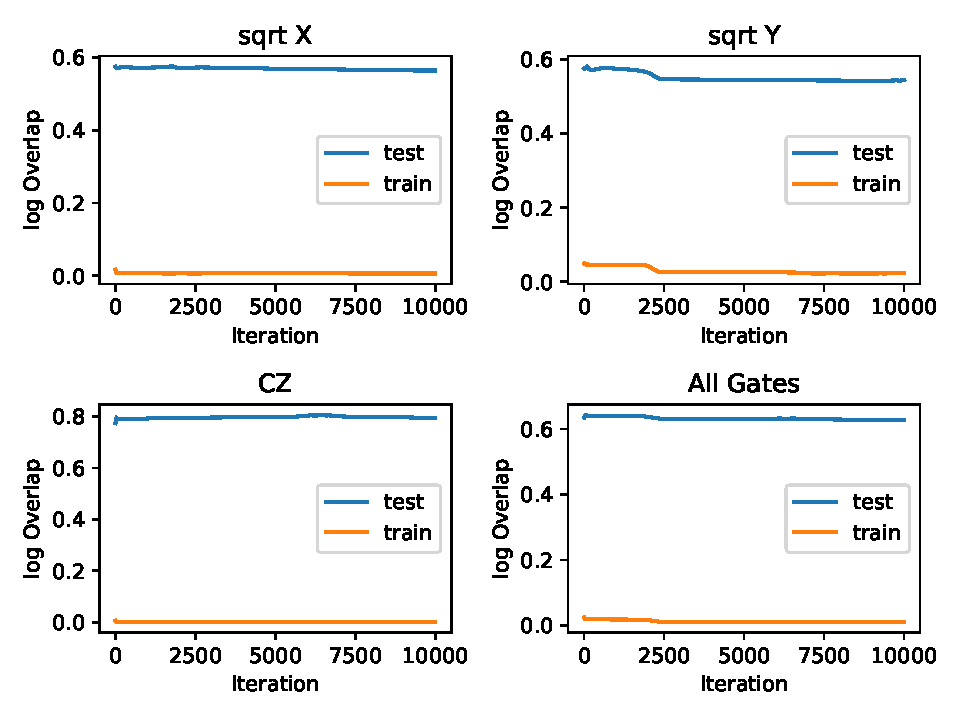
\includegraphics[width=\textwidth]{figures/results/SR-restarts-learned/avgOverlap_8.pdf}
  \caption[Training Overlap of Stochastic Reconfiguration with Restarts Learned]{Training 
  Overlap of Stochastic Reconfiguration with Restarts and the $CZ$ gates learned for 8 samples.}
  \label{fig:sr_restarts_overlap_8}
\end{figure}

For 47 samples, the change in the average training and test overlap is fluctuating during all 10,000
training iterations on all gates. For the 
$\sqrt{X}$ gate, the log overlap on the test set steadily decreases from 
about $0.35$ to about $0.30$. In the same period, the overlap on the training data decreases from about $0.24$ to about $0.21$.

For the $\sqrt{Y}$ gate, the training and test overlaps decrease by about $0.50$ within the first few iterations. 
Afterward, the training overlap slightly increases until about the 2,500th iteration before it decreases again 
until the 10,000th iteration. On the test data, the overlap follows a similar pattern. The 
training overlap is slightly below $0.275$ after 10,000 iterations. The test overlap is at about $0.325$ 
at the end of the 10,000 iterations. 

For the $CZ$ gate, there is an initial drop in the training and testing overlaps. Afterward, 
the training overlap oscillates at around $0.5$ for the first 5.00 iterations before it slowly increases to about 
0.10 after 10,000 iterations. The test overlap oscillates around about 0.16 for the first 5,000 iterations and 
slowly increases to about 0.17 within the following 5,000 iterations. 

Averaged over all gates, the training and test error both drop within the first few iterations to about 
0.20 on the test data and about 0.27 on the training data. Afterward, the overlap slowly decreases to about 0.19 and 
0.24 over the period of 10,000 iterations.

The training and test overlap follows similar pattern for 43, 50, and 54 samples. For 43 samples, the 
overlap is less fluctuating for the $\sqrt{X}$ gate. It reaches lower values on the $\sqrt{Y}$ gate with 
a final testing overlap of about 0.30. The overall overlap on all gates is also lower with about 0.25.

For 50 samples, the final testing overlap is lower for the single qubit gates with about 0.24 on the $\sqrt{X}$
and 0.28 on the $\sqrt{Y}$ gate. The final test overlap is with about 0.15 similar for the $CZ$ gate. On all gates, 
the average final test overlap is about 0.23 with 50 samples.

With 54 samples, the testing overlap on the $\sqrt{X}$ goes down to about 0.23. On the $\sqrt{Y}$ gate it goes 
down to about 0.24, and to about 0.12 on the $CZ$ gate. Over all gate, the testing overlap reaches a value of about 
0.20 after 10,000 iterations when trained with 50 samples.

The graphs for 43, 50, and 54 qubits are included in the appendix.

\begin{figure}[H]
  \centering
  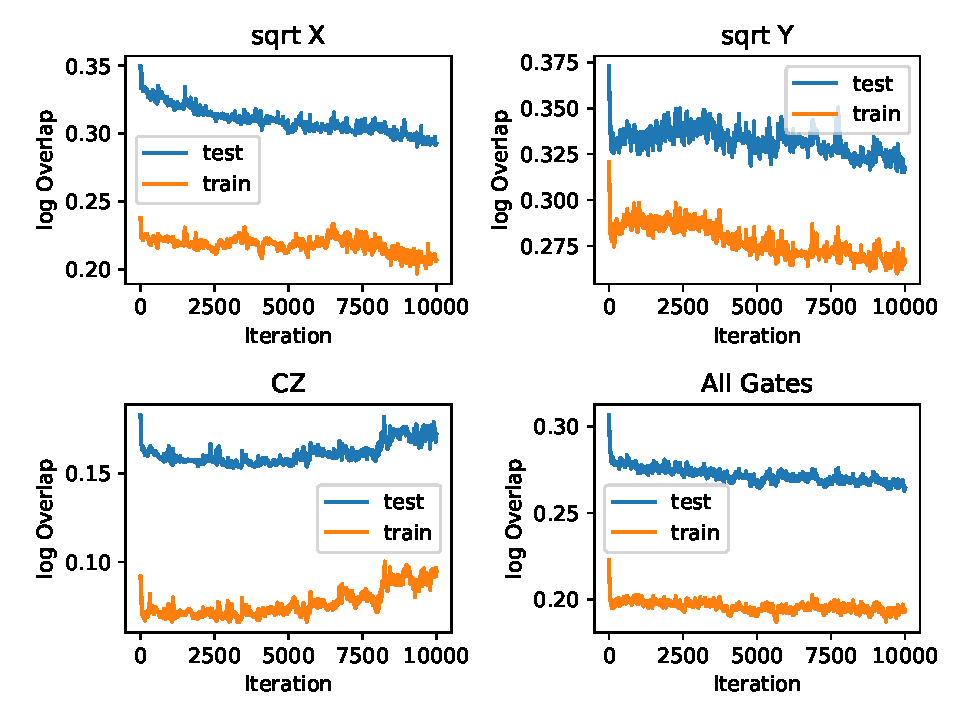
\includegraphics[width=\textwidth]{figures/results/SR-restarts-learned/avgOverlap_47.pdf}
  \caption[Training Overlap of Stochastic Reconfiguration with Restarts Learned]{Training 
  Overlap of Stochastic Reconfiguration with Restarts Learned for 47 samples.}
  \label{fig:sr_restarts_overlap_47}
\end{figure}

With 303 samples, the mean test and training overlaps oscillate even more. The overlap on the training and the 
test data is very close. 

For the $\sqrt{X}$ gate, the overlap drops from about 0.28 to 0.23 within the first very few iterations. 
Afterward, it slowly decreases further to about 0.22 throughout the 10,000 iterations.

On the $\sqrt{Y}$ gate, the overlap has the biggest decrease from about 0.28 to 0.25 within the first 
few iterations. Afterward, it keeps steady to about the 2,500th iteration before it drops to 0.24 at about 5,000 iterations.
Then, it increases again to about 0.255 at about 7,500 iterations and stays in that range for the remaining iterations.

On the $CZ$ gate, the overlap starts at about 0.09 and drops to about 0.06 within the first few iterations. 
For the remaining training process, it slowly increases again to about 0.07. 

Averaged over all gates, the training and testing overlap is about 0.22 at the beginning of the training, 
drops to 0.19 within the first very few iterations and hits a minimum of about 0.18 at about 6,000 iterations before 
it increases again. Starting at about 9,000 iterations, it decreases again to about 0.18.

\begin{figure}[H]
  \centering
  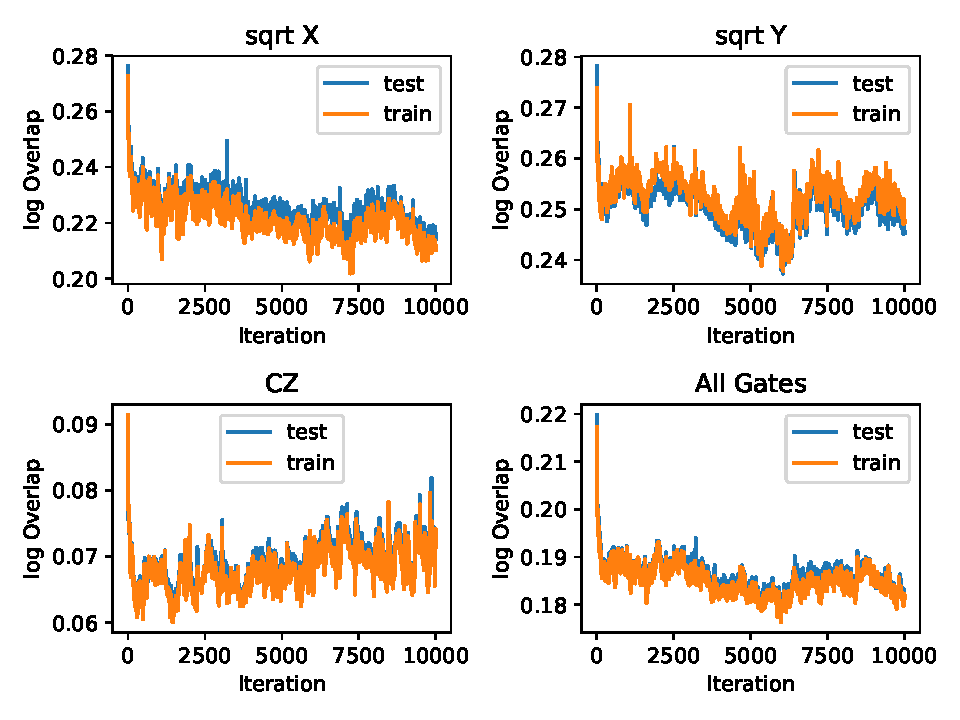
\includegraphics[width=\textwidth]{figures/results/SR-restarts-learned/avgOverlap_303.pdf}
  \caption[Training Overlap of Stochastic Reconfiguration with Restarts Learned]{Training 
  Overlap of Stochastic Reconfiguration with Restarts and the $CZ$ gates learned for 303 samples.}
  \label{fig:sr_restarts_overlap_303}
\end{figure}

\newpage

\subsection{Stochastic Reconfiguration without Random Restarts and CZ Gates Learned}

The last section showed the results for RBMs that were trained with the Stochastic Reconfiguration
method and random restarts. The following section shows the results of RBMs trained without restarts.

Figure~\ref{fig:sr_no_restarts_avgPDF} shows the averaged output distribution of all RBMs and
the averaged true output distributions of all circuits. As before, the 
true output distributions approach a Porter-Thomas shape with an increasing number of cycles.
The TVD of the average output of all RBMs trained with SR without restarts
is 0.34 for 5, 0.38 for 10, 0.34 for 15, and 0.38 for 20 cycles. The corresponding cross entropy is 
0.12 for 5, 0.00 for 10, 0.04 for 15, and 0.00 for 20 cycles.

\begin{figure}[H]
  \centering
  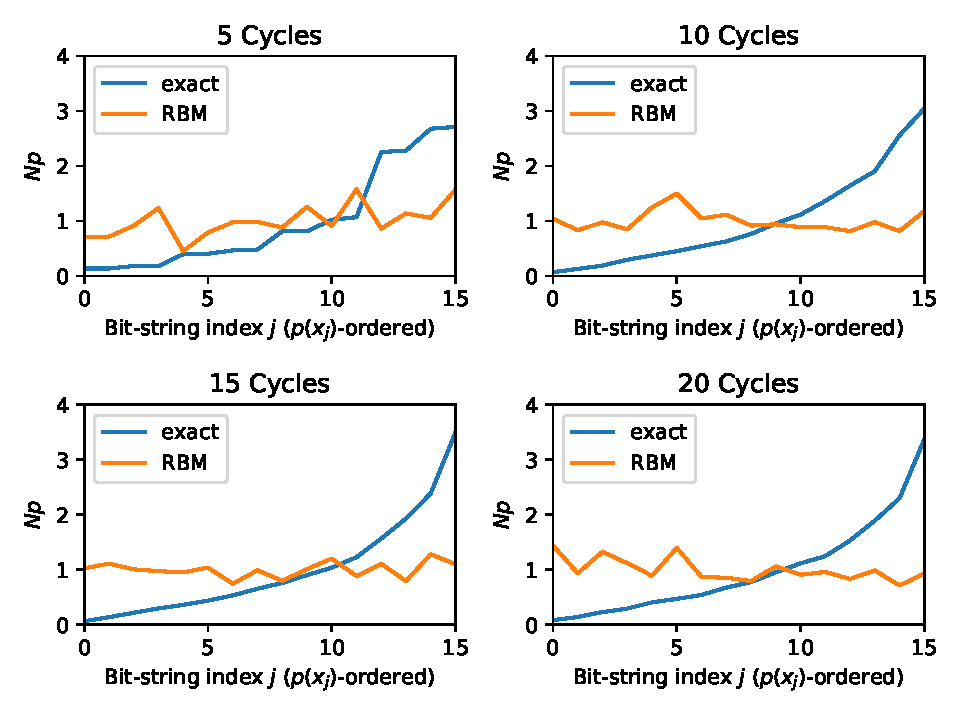
\includegraphics[width=\textwidth]{figures/results/SR-no-restarts-learned/avgPDF.pdf}
  \caption[Scaled average output probabilities of Stochastic Reconfiguration without Restarts Learned]{
    Scaled average output probabilities of Stochastic Reconfiguration without Restarts Learned. The true 
    output distribution approaches a Porter-Thomas shape with increasing number of cycles.}
  \label{fig:sr_no_restarts_avgPDF}
\end{figure}

In figure~\ref{fig:sr_no_restarts_bestPDF}, only the output distribution of the best performing RBMs with respect to the 
TVD are selected and their outputs averaged. The averaged best output distribution for the SR methods without 
random restarts and $CZ$ gates learned has a TVD of 0.07 for 5, 0.18 for 10, 0.21 for 15, and 0.21 for 20 
cycles. The cross entropy fidelity is 0.71 for 5, 0.37 for 10, 0.40 for 15, and 0.35 for 20 cycles each. 

\begin{figure}[H]
  \centering
  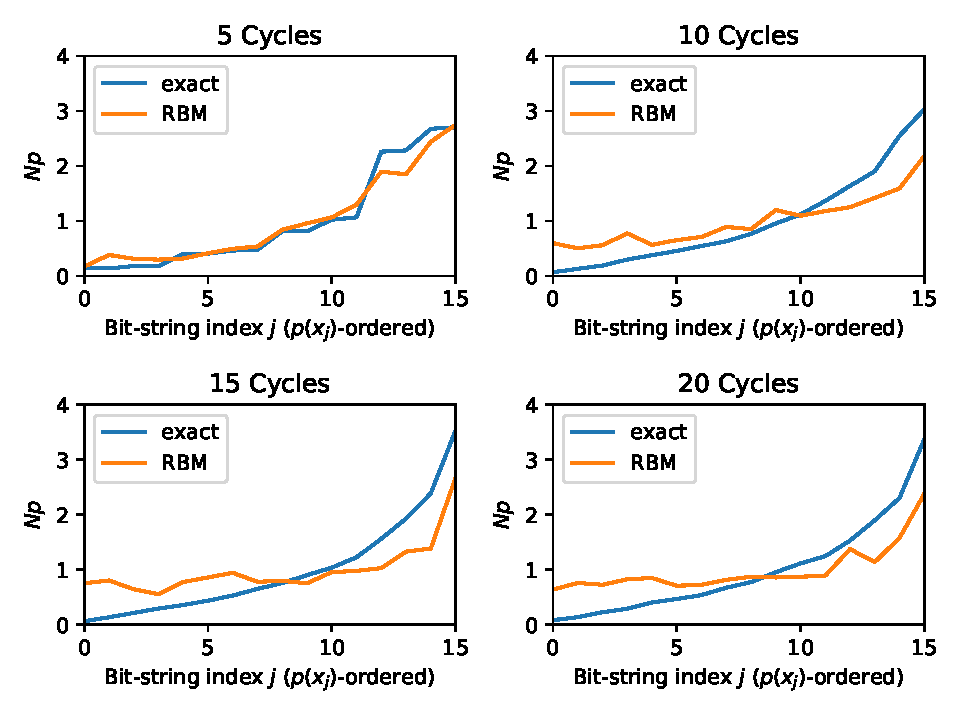
\includegraphics[width=\textwidth]{figures/results/SR-no-restarts-learned/avgBestPDF.pdf}
  \caption[Averaged best performing scaled output probabilities of Stochastic Reconfiguration without Restarts Learned]{
    Scaled average output probabilities of Stochastic Reconfiguration without Restarts Learned, only RBMs with lowest
    TVD for each circuit are considered. The true 
    output distribution approaches a Porter-Thomas shape with increasing number of cycles.}
  \label{fig:sr_no_restarts_bestPDF}
\end{figure}

Figure~\ref{fig:sr_no_restarts_tvd} and figure~\ref{fig:sr_no_restarts_fxeb} give a more detailed overview of the influence of the 
number of training samples and training iterations on the TVD and cross entropy fidelity achieved by 
the RBMs. Also here, there seems to be no correlation between the number of training
iterations and the performance of the RBMs. 

For 5 cycles, a higher number of training samples 
correlates with an overall lower TVD for 10,000 and 100,000 iterations, but not so for 1,000 iterations. The RBM performs best on 
circuits with a depth of 5 cycles when trained with 100,000 iterations and 303 samples. In this case, 
it achieves a mean TVD of $0.43$. Overall, the performance is independent of the number of 
training iterations when trained with less than 303 samples. In these cases, the performance is very 
similar for 1,000, 10,000, and 100,000 iterations. The only exception is for 54 samples, where 100,000 iterations lead to a 
mean TVD of $0.55$, while the mean TVD is at $0.64$ when trained with 1,000. the mean TVD is $0.62$ when trained for 
10,000 iterations. 

For 10 cycles, 1,000 training iterations achieves the lowest TVDs for 43 or more samples. 
100,000 iterations lead to a lower TVD than 10,000 iterations in all cases. 

For 15 and 20 cycles, again 10,000 training iterations correlate with the highest TVD in most cases.
The performance is similar for all number of training samples. The lowest TVDs are achieved when trained for 1,000
iterations. Also in these cases, the performance is similar for all tested number of training samples; with 
the exception that it is significantly higher for 8 samples.

\begin{figure}[H]
  \centering
  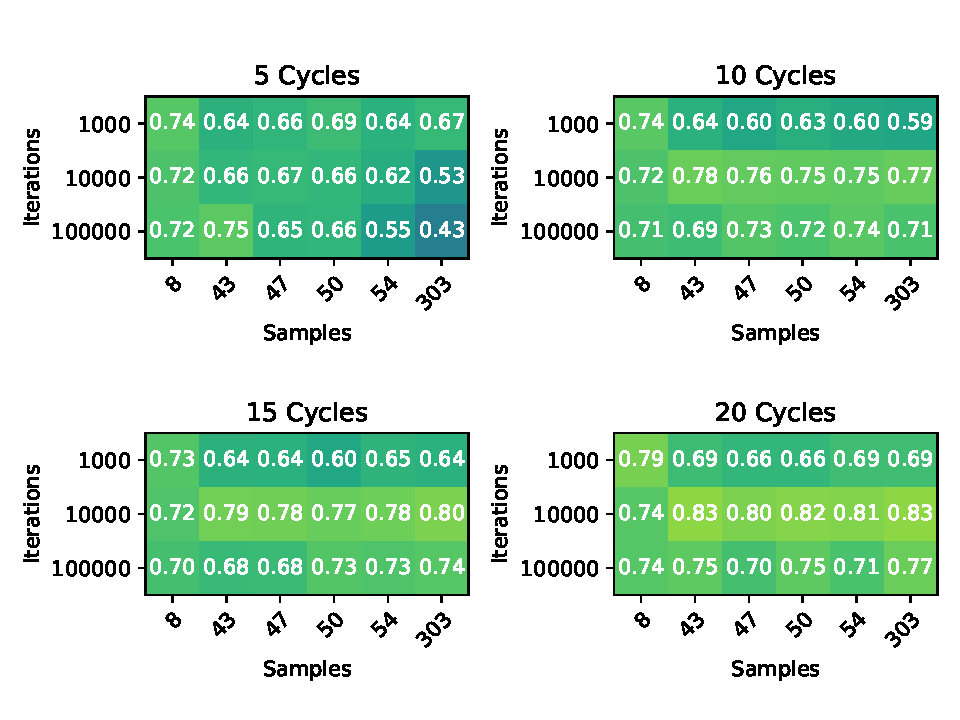
\includegraphics[width=\textwidth]{figures/results/SR-no-restarts-learned/tvd_heatmap.pdf}
  \caption[TVD of Stochastic Reconfiguration without Restarts Learned]{TVD of Stochastic 
  Reconfiguration without Restarts Learned for the combinations of iterations and samples tested.
  For 100,000 iterations and 303 samples, the experiments did not finish within the time limit.}
  \label{fig:sr_no_restarts_tvd}
\end{figure}

As in the case with restarts, a lower TVD does not always correlate with a higher cross entropy fidelity as 
figure~\ref{fig:sr_no_restarts_fxeb}
implies. For 5 cycles, the highest fidelity is achieved with 303 samples and 10,000 iterations, on 10 cycles 
with 43 samples and 1,000 iterations, with 47 samples and 100,000 iterations on 15 cycles, and with 303 samples and 
0,000 iterations on 20 cycles. There is no clear tendency that shows a correlation between 
the number of training iterations, samples, and cross entropy fidelity.

\begin{figure}[H]
  \centering
  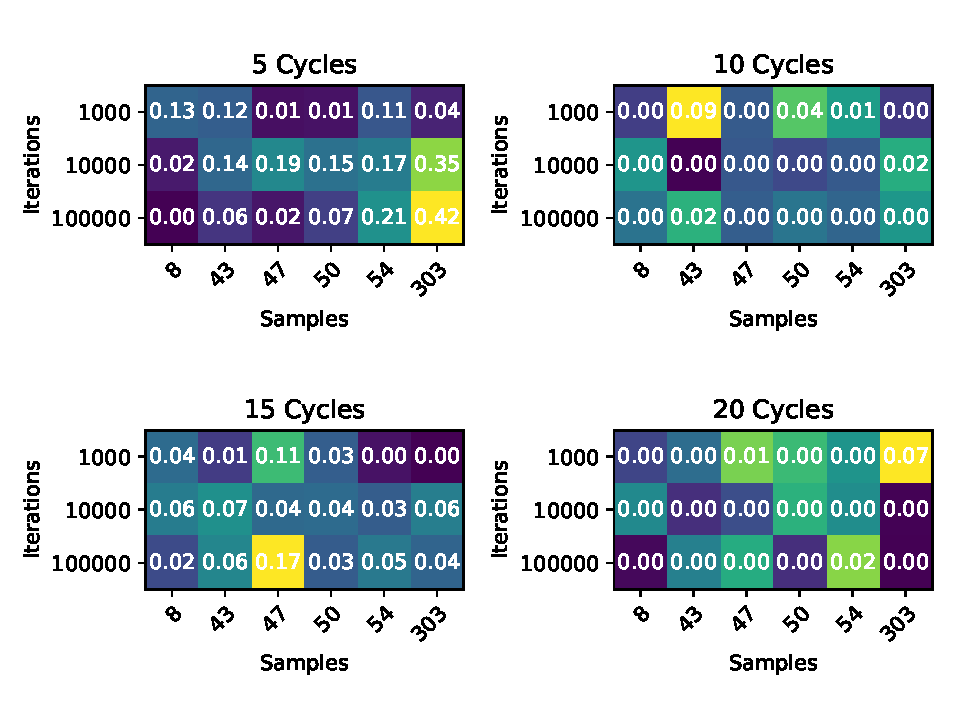
\includegraphics[width=\textwidth]{figures/results/SR-no-restarts-learned/fxeb_heatmap.pdf}
  \caption[Cross-entropy Fidelity of Stochastic Reconfiguration without Restarts Learned]{Cross-entropy Fidelity of Stochastic 
  Reconfiguration without Restarts Learned for the combinations of iterations and samples tested.
  For 100,000 iterations and 303 samples, the experiments did not finish within the time limit.}
  \label{fig:sr_no_restarts_fxeb}
\end{figure}

Figure~\ref{fig:sr_no_restarts_overlap_8} to~\ref{fig:sr_no_restarts_overlap_303} detail the mean log overlap of the RBMs during the 
training process when trained with 10,000 iterations for 8, 47, and 303 samples. The 
mean overlap of the RBM's state and the distribution implied by the training and test data sets are measured 
for each training iteration.

For 8 samples, the log overlap on the training set can be reduced to about 0 for all three gates after about 2,500 iterations.
For the $\sqrt{Y}$ gate, the overlap plateaus at about 0.1 after about 1,000 iterations, before it starts 
to decrease again from 2,000 iterations on. 

The log overlap on the test goes down to about $0.50$ for the $\sqrt{X}$ gate within the first 500 iterations and stays at 
that level for the remaining training process. For the $\sqrt{Y}$ gate, the testing overlap decreases to about 
$0.55$ within the first about 500 iterations. Afterward, it increases again to about 0.60 where it stays for the 
remaining iterations. For the $CZ$ gate, it goes down to about 1.0 within the first 500 iterations and stays at 
that level afterward.

Averaged over all gates, the overlap goes down close to 0 within the first 2,500 training iterations. 
After 500 iterations, the test 
overlap reaches about 0.65 at which it stays for the remaining training iterations. It only 
slightly increases again over the course of the next about 2,000 iterations.


\begin{figure}[H]
  \centering
  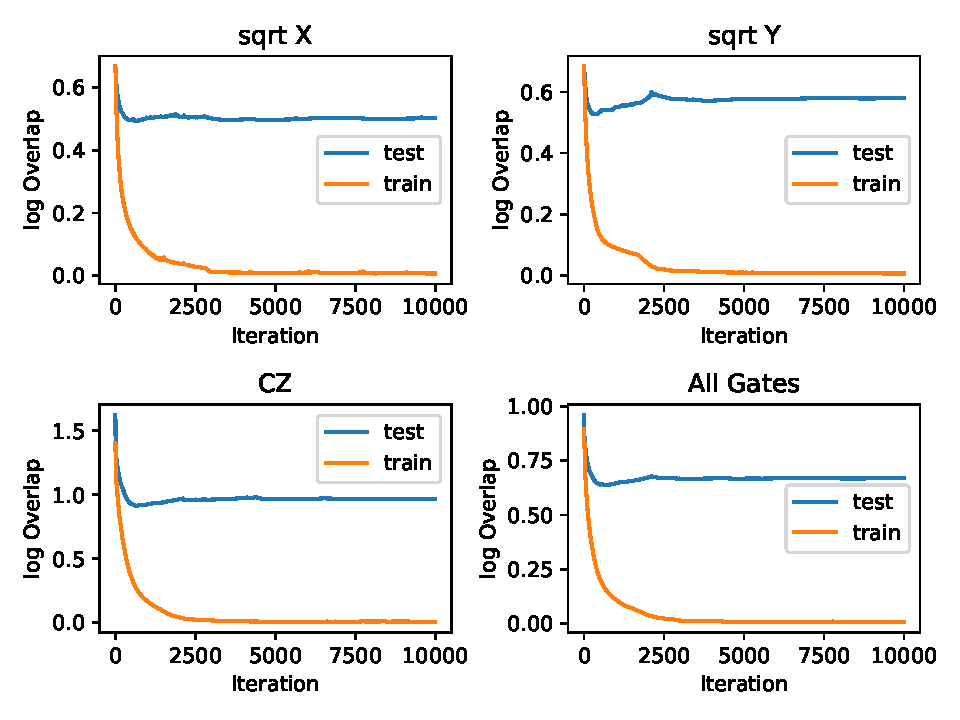
\includegraphics[width=\textwidth]{figures/results/SR-no-restarts-learned/avgOverlap_8.pdf}
  \caption[Training Overlap of Stochastic Reconfiguration without Restarts Learned]{Training 
  Overlap of Stochastic Reconfiguration without Restarts Learned for 8 samples.}
  \label{fig:sr_no_restarts_overlap_8}
\end{figure}

For 47 samples, the change in the average training and test overlap is slightly more fluctuating than for 8 qubits. For the 
$\sqrt{X}$ gate, the log overlap on the training set steadily decreases on the test data set from 
about $0.70$ to about $0.19$ within the first 2,500 training iterations. The overlap on the test data 
decreases to about 0.25 within the same time. Afterward, the training overlap increases again to about 
0.20 within the next 1,500 iterations. At the same time, the overlap on the test data increases to about 
0.3 and stays at that level.

On the $\sqrt{Y}$ gate, the training overlap decreases to about 0.20 within the first 2,500 training iterations 
and stays at that level from thereon. The test overlap decreases to about 0.29 within the first 2,500 iterations 
and also stays there for the remaining part of the training process.

On the $CZ$ gate, the training overlap decreases to about 0.1 in the first 3,000 training iterations. It does 
not change much afterward. The overlap on the test data goes down to about 0.2 within the first 3,500 iterations 
and stays at that level.

Averaged over all gates, the overlap on the test data goes down to about 0.18 within the first 2,500 training iterations. 
The test overlap goes down to about 0.25 in the same time. Both metrics stay at those values afterward.

The training and test overlap follows similar pattern for 43, 50, and 54 samples with the 
test overlap being closer to the training overlap with increasing number of samples. The overall
testing overlap averaged over all gates approaches 0.2 for 54 samples.

The graphs for 43, 50, and 54 qubits are included in the appendix.

\begin{figure}[H]
  \centering
  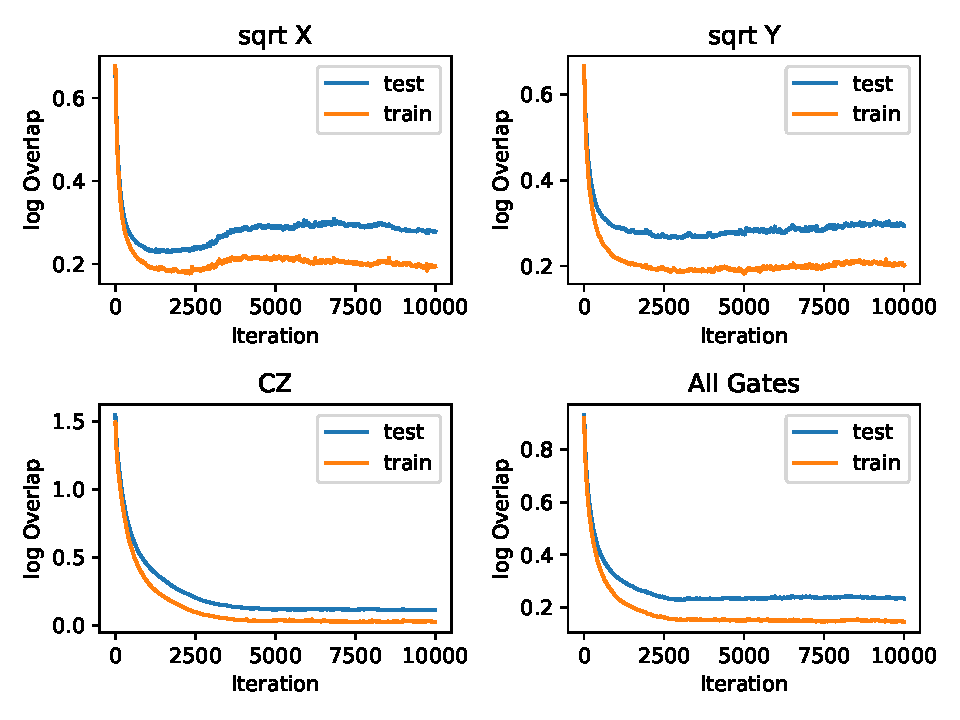
\includegraphics[width=\textwidth]{figures/results/SR-no-restarts-learned/avgOverlap_47.pdf}
  \caption[Training Overlap of Stochastic Reconfiguration without Restarts Learned]{Training 
  Overlap of Stochastic Reconfiguration without Restarts Learned for 47 samples.}
  \label{fig:sr_no_restarts_overlap_47}
\end{figure}

With 303 samples, the curves of the log overlap on the training data look very similar to the 
ones with 47 samples. A noticeable difference can be observed for the test overlap, which is 
about the same as the training overlap in all cases.

\begin{figure}[H]
  \centering
  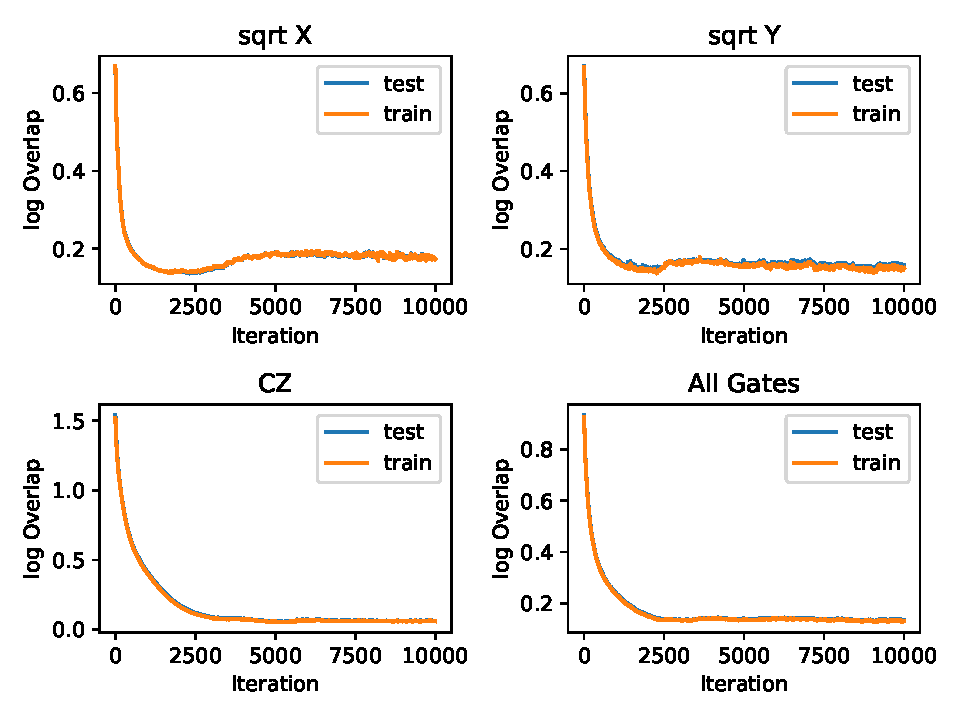
\includegraphics[width=\textwidth]{figures/results/SR-no-restarts-learned/avgOverlap_303.pdf}
  \caption[Training Overlap of Stochastic Reconfiguration without Restarts Learned]{Training 
  Overlap of Stochastic Reconfiguration without Restarts Learned for 303 samples.}
  \label{fig:sr_no_restarts_overlap_303}
\end{figure}

\newpage

\subsection{Stochastic Reconfiguration with Random Restarts and CZ Gates Applied Exactly}

In previous works, the $CZ$ gate had been applied to the RBM state exactly \cite{jnsson2018neuralnetwork}. This study compares 
the performance of RBMs when the $CZ$ gate is applied exactly and learned. The comparison might shed
light on how the training process of a gate is influenced by the number of qubits the gate 
is acting on. It further can give a hint on whether the addition of hidden units by applying the $CZ$
gate exactly influences the training process of the other gates.
The following section shows the results of RBMs trained with restarts and the $CZ$ gates applied 
with the rules from section X.

Figure~\ref{fig:sr_exact_avgPDF} shows the averaged output distribution of all RBMs and
the averaged true output distributions of all circuits. As in the cases before, the 
true output distributions approach a Porter-Thomas shape with an increasing number of cycles.
The TVD of the average output of all RBMs 
is 0.35 for 5, 0.33 for 10, 0.34 for 15, and 0.38 for 20 cycles. The corresponding cross entropy is 
0.20 for 5, 0.02 for 10, 0.06 for 15, and 0.00 for 20 cycles.

\begin{figure}[H]
  \centering
  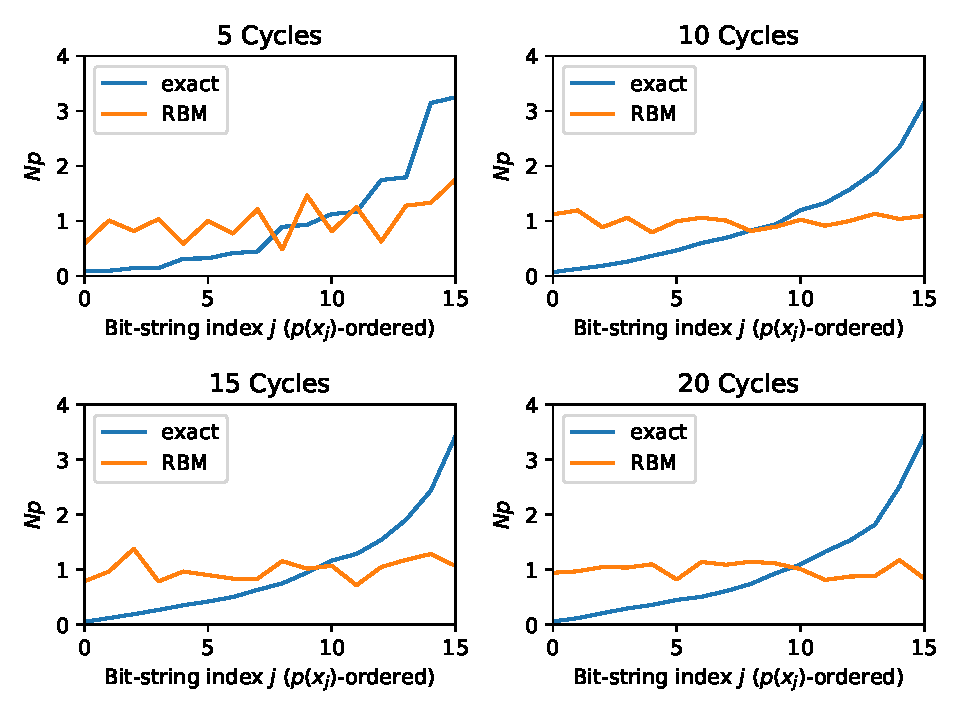
\includegraphics[width=\textwidth]{figures/results/SR-restarts-not-learned/avgPDF.pdf}
  \caption[Scaled average output probabilities of Stochastic Reconfiguration with Restarts Exact]{
    Scaled average output probabilities of Stochastic Reconfiguration with Restarts Exact. The true 
    output distribution approaches a Porter-Thomas shape with increasing number of cycles.}
  \label{fig:sr_exact_avgPDF}
\end{figure}

In figure~\ref{fig:sr_exact_bestPDF}, only the output distribution of the best performing RBMs with respect to the 
TVD are selected. Their outputs are averaged. The averaged best output distribution 
has a TVD of 0.03 for 5, 0.13 for 10, 0.22 for 15, and 0.21 for 20 
cycles. The cross entropy fidelity is 1.00 for 5, 0.46 for 10, 0.33 for 15, and 0.40 for 20 cycles each. 


\begin{figure}[H]
  \centering
  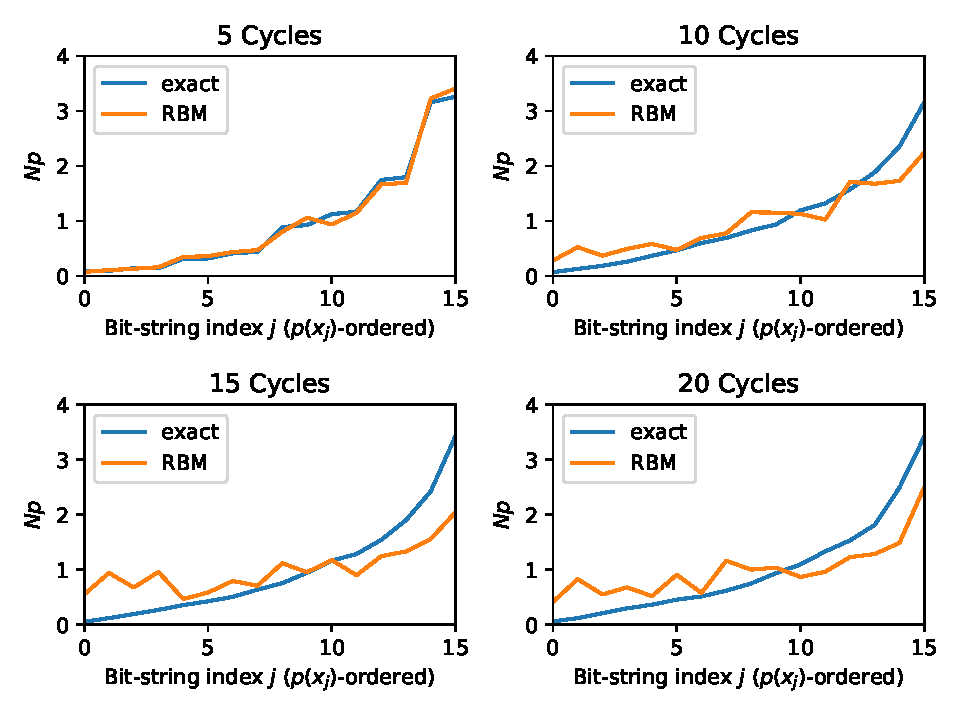
\includegraphics[width=\textwidth]{figures/results/SR-restarts-not-learned/avgBestPDF.pdf}
  \caption[Averaged best performing scaled output probabilities of Stochastic Reconfiguration with Restarts Exact]{
    Scaled average output probabilities of Stochastic Reconfiguration with Restarts Exact, only RBMs with lowest
    TVD for each circuit are considered. The true 
    output distribution approaches a Porter-Thomas shape with increasing number of cycles.}
  \label{fig:sr_exact_bestPDF}
\end{figure}

Figure~\ref{fig:sr_exact_tvd} and figure~\ref{fig:sr_exact_fxeb} detail the influence of the 
number of training samples and training iterations on the TVD and cross entropy fidelity achieved by 
the RBMs. 

For 5 cycles, a higher number of training samples 
correlates with an overall lower TVD. The RBM performs best on 
circuits with a depth of 5 cycles when trained with 100,000 iterations and 303 samples. In that case, 
it achieves a mean TVD of $0.49$. Overall, the performance is similar for 1,000 and 100,000 iterations.

For 10 cycles, the lowest TVD is also achieved by RBMs trained with 303 samples and 100,000 iterations.
A higher number of samples correlates with an overall lower TVD for 100,000 iterations. For 1,000 iterations, 
the TVD is about 0.60 for 43 samples and higher; and 0.74 for 8 samples. For 10,000 iterations, the TVD varies 
around about 0.75 independent of the number of samples. 

For 15 and 20 cycles, 10,000 training iterations correlate with the highest TVD in most cases.
The performance is similar for all numbers of training samples. The lowest TVDs are achieved with 100,000
iterations and 47 or 54 samples. With 10,000 iterations, a higher number of training samples correlates 
with a higher TVD. For 1,000 and 100,000 iterations, there is no clear difference in the number of training 
samples.

\begin{figure}[H]
  \centering
  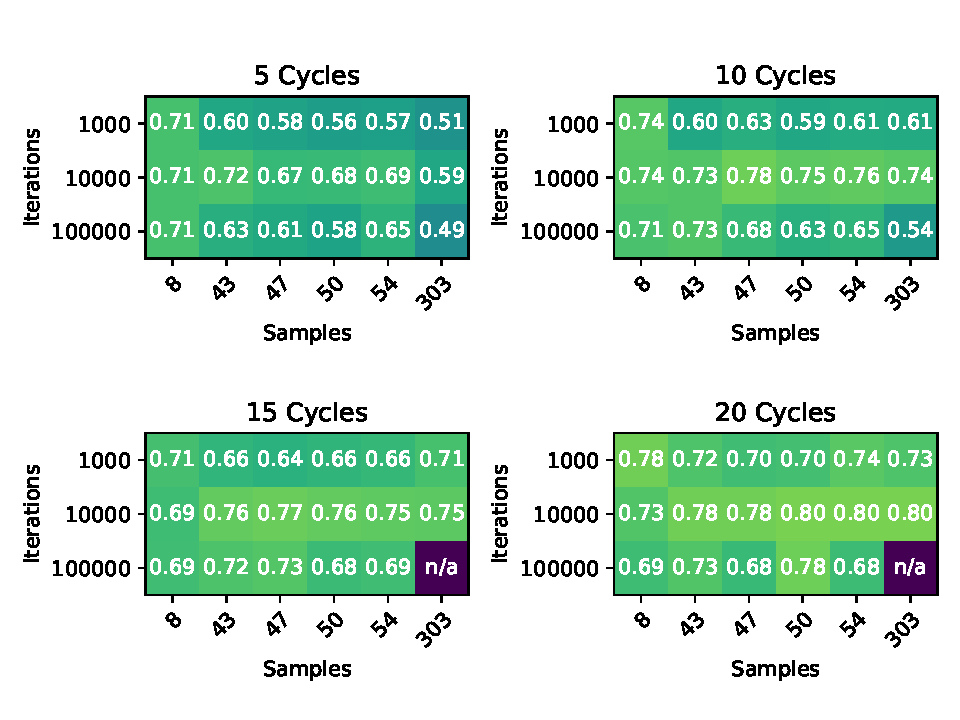
\includegraphics[width=\textwidth]{figures/results/SR-restarts-not-learned/tvd_heatmap.pdf}
  \caption[TVD of Stochastic Reconfiguration with Restarts Exact]{TVD of Stochastic 
  Reconfiguration with Restarts Exact for the combinations of iterations and samples tested.
  For 100,000 iterations and 303 samples, the experiments did not finish within the time limit.}
  \label{fig:sr_exact_tvd}
\end{figure}

Figure~\ref{fig:sr_no_restarts_fxeb} shows the average cross entropy fidelity achieved. On 5 and 10
cycles, the highest fidelity is achieved with 303 samples and 100,000 iterations. 
For 15 cycles, the highest fidelity is achieved with 50 samples on 100,000 iterations and 
303 samples and 10,000 iterations.
For 20 cycles, the highest fidelity is achieved on RBMs trained with 47 samples for 100,000 iterations.
There is no clear tendency that shows a correlation between 
the number of training iterations or samples and the cross entropy fidelity.

\begin{figure}[H]
  \centering
  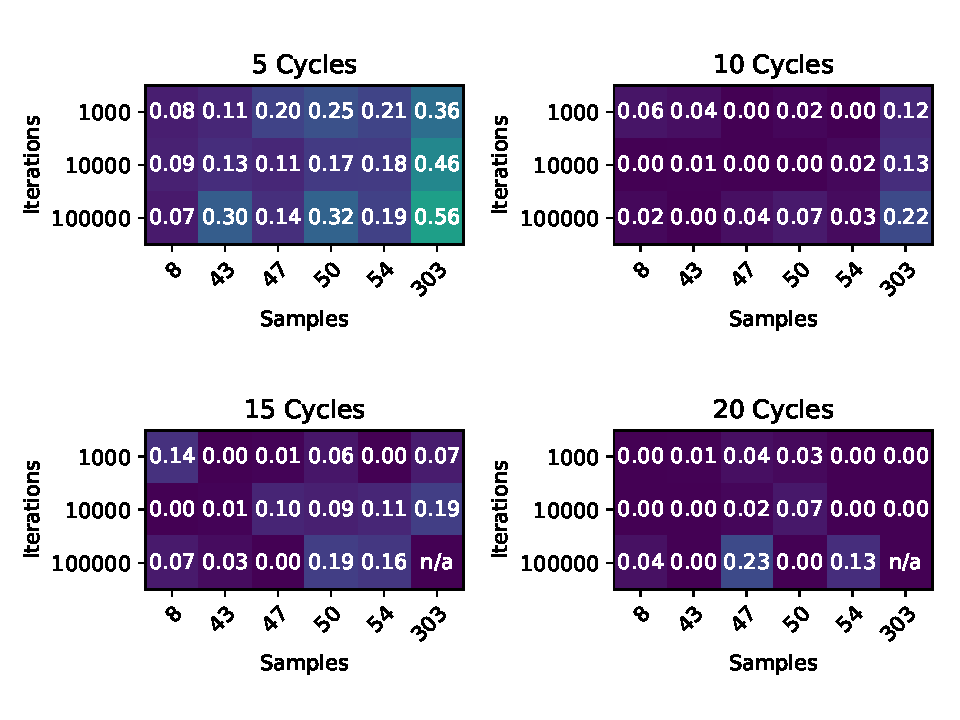
\includegraphics[width=\textwidth]{figures/results/SR-restarts-not-learned/fxeb_heatmap.pdf}
  \caption[Cross-entropy Fidelity of Stochastic Reconfiguration with Restarts Exact]{Cross-entropy Fidelity of Stochastic 
  Reconfiguration with Restarts Exact for the combinations of iterations and samples tested.
  For 100,000 iterations and 303 samples, the experiments did not finish within the time limit.}
  \label{fig:sr_exact_fxeb}
\end{figure}

Figure~\ref{fig:sr_exact_overlap_8} to~\ref{fig:sr_exact_overlap_303} detail the mean log overlap of the RBMs during the 
training process when trained with 10,000 iterations for 8, 47, and 303 samples. The 
mean overlap of the RBM's state and the distribution implied by the training and test data sets are measured 
for each training iteration.

For 8 samples, both the training and the testing overlap don't vary much during the training. The training errors on the $\sqrt{X}$ and 
$\sqrt{Y}$ gate are both close to 0 during the whole training process. The test error is about 0.60.

\begin{figure}[H]
  \centering
  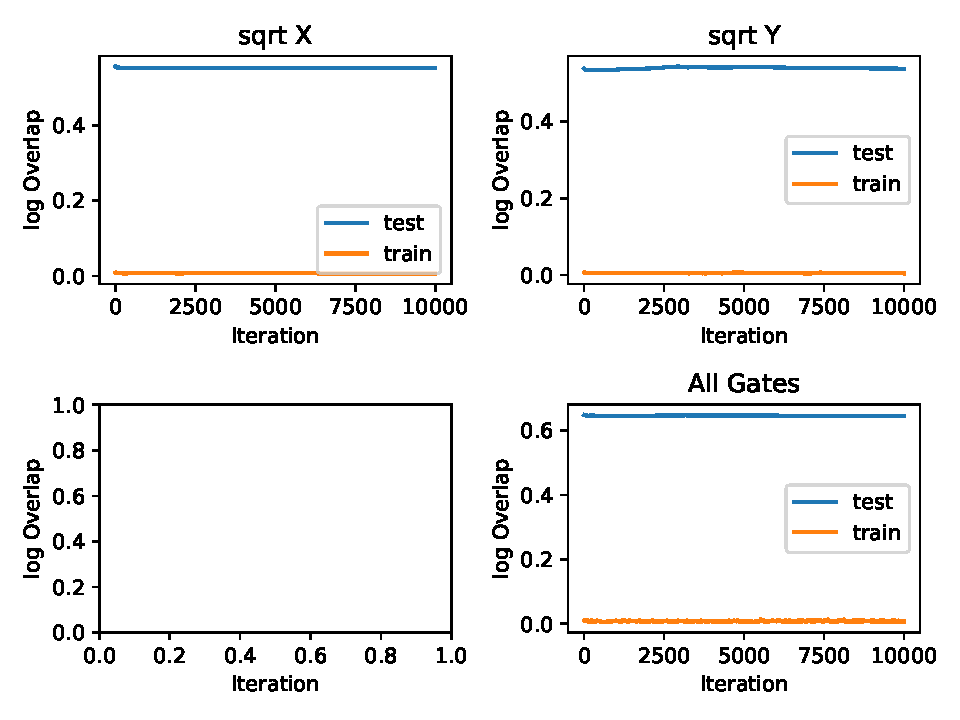
\includegraphics[width=\textwidth]{figures/results/SR-restarts-not-learned/avgOverlap_8.pdf}
  \caption[Training Overlap of Stochastic Reconfiguration with Restarts Exact]{Training 
  Overlap of Stochastic Reconfiguration with Restarts Exact for 8 samples.}
  \label{fig:sr_exact_overlap_8}
\end{figure}

For 47 samples, the change in the average training and test overlap is oscillating. For the 
$\sqrt{X}$ gate, the log overlap on the training set oscillates around about 0.16 during most 
of the training process. It 
reaches its lowest value of about 0.13 after 3,000 iterations. The overlap on the test data 
oscillates around about 0.21 during the whole process. The training error drops from 
0.175 to 0.16 within the first few iterations. The training overlap drops from 0.25 to 0.21 at that time.

On the $\sqrt{Y}$ gate, the training overlap decreases to about 0.17 within the first few training iterations 
and oscillates around that value from thereon. The test overlap decreases to about 0.28 within the first few
iterations and slowly increases to about 0.3 throughout the training process.

The training and test overlap follows similar pattern for 43, 50, and 54 samples.
With 43 samples, the overlaps oscillate less for the $\sqrt{X}$ gate. The testing overlap is about 
0.33 for 43 samples on the $\sqrt{X}$ while the training overlap oscillates around about 0.19.
On the $\sqrt{Y}$ gate, the training overlap is at about 0.16 as for 47 samples. The testing overlap is 
lower and reaches a value of about 0.23 after 10,000 iterations. The averaged testing overlap is higher than 
for 47 samples with a value of about 0.27 and the training overlap is similar with a value of about 0.15.

With 50 and 53 samples, the testing overlap is higher in both cases for the $\sqrt{X}$ gate than for 
47 samples. It is at about 0.29 for 50 samples and about 0.33 for 53 samples. The training overlap is about 
0.21 for 50 samples and about 0.25 for 53 samples on that gate.

On the $\sqrt{Y}$ gate, the testing overlap is with a value of about 0.25 lower in both cases. The 
training overlap on that gate is about 0.18 in both cases. Averaged over both gates, the training 
overlap gets reduced to about 0.18 in both cases while the testing overlap goes down to about 0.25 
throughout the 10,000 iterations.

The graphs for 43, 50, and 54 qubits are included in the appendix.

\begin{figure}[H]
  \centering
  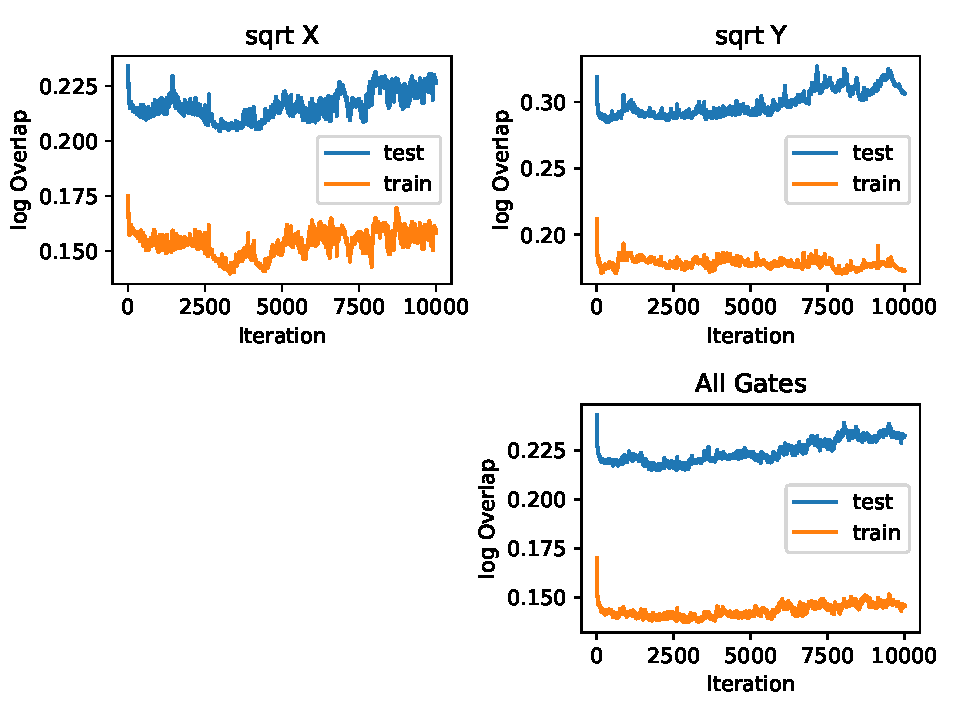
\includegraphics[width=\textwidth]{figures/results/SR-restarts-not-learned/avgOverlap_47.pdf}
  \caption[Training Overlap of Stochastic Reconfiguration with Restarts Exact]{Training 
  Overlap of Stochastic Reconfiguration with Restarts Exact for 47 samples.}
  \label{fig:sr_exact_overlap_47}
\end{figure}

With 303 samples, the oscillation in the test and training overlap is even more than for 47 samples. 
For the $\sqrt{X}$ gate, both values drop to about 0.21 within the first 1,000 training iterations. 
Afterward, the overlaps increase to about 0.25 at 6,000 iterations. It decrease to about 0.24 in the 
remaining part of the training process again.

The process looks similar for the $\sqrt{Y}$ gate. The overlap goes down to about 0.22 within the 
first 1,000 iterations. Afterward, it goes up to about 0.24 again and stays at that level for the 
following training iterations.

\begin{figure}[H]
  \centering
  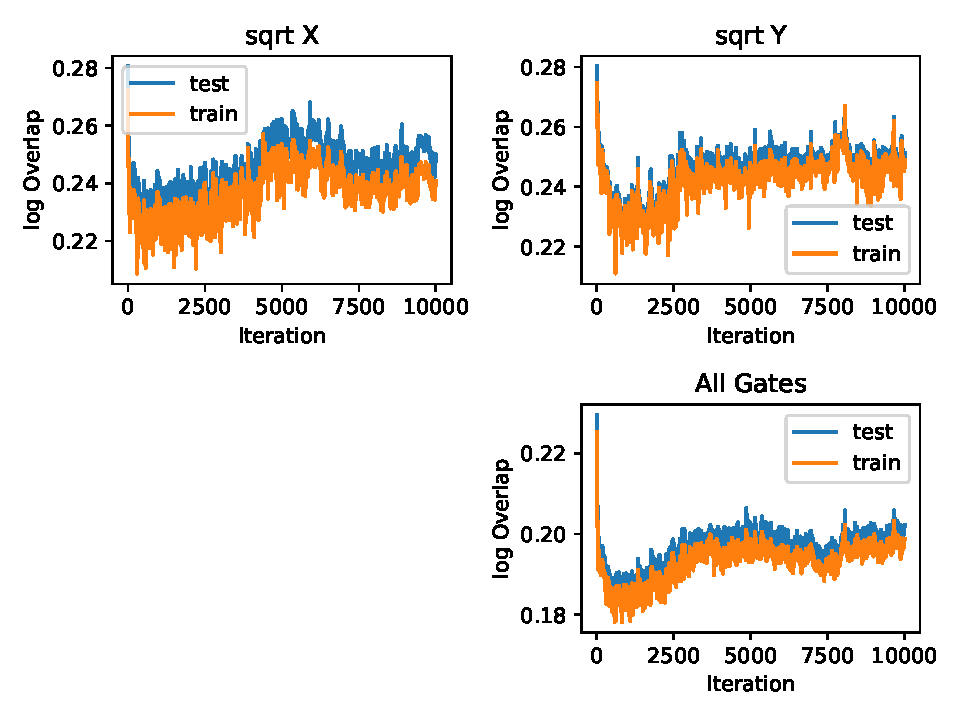
\includegraphics[width=\textwidth]{figures/results/SR-restarts-not-learned/avgOverlap_303.pdf}
  \caption[Training Overlap of Stochastic Reconfiguration with Restarts Exact]{Training 
  Overlap of Stochastic Reconfiguration with Restarts Exact for 303 samples.}
  \label{fig:sr_exact_overlap_303}
\end{figure}

\newpage

\subsection{AdaMax with Random Restarts and CZ Gates Learned}

AdaMax had also been used for training RBMs for the 
classical simulation of quantum circuits before \cite{jnsson2018neuralnetwork}. The following section presents the results
of RBMs trained with AdaMax and five random restarts. The $CZ$ gates are also applied with the 
learning approach in these cases.

Figure~\ref{fig:am_avgPDF} shows the averaged output distribution of all RBMs trained with AdaMax and 
the averaged true output distributions of all circuits. As in the other cases, the 
true output distributions approach a Porter-Thomas shape with an increasing number of cycles.
The TVD of the average output of all RBMs trained with AdaMax
is 0.25 for 5, 0.30 for 10, 0.35 for 15, and 0.33 for 20 cycles. The corresponding cross entropy is 
0.20 for 5, 0.08 for 10, 0.06 for 15, and 0.04 for 20 cycles.

\begin{figure}[H]
  \centering
  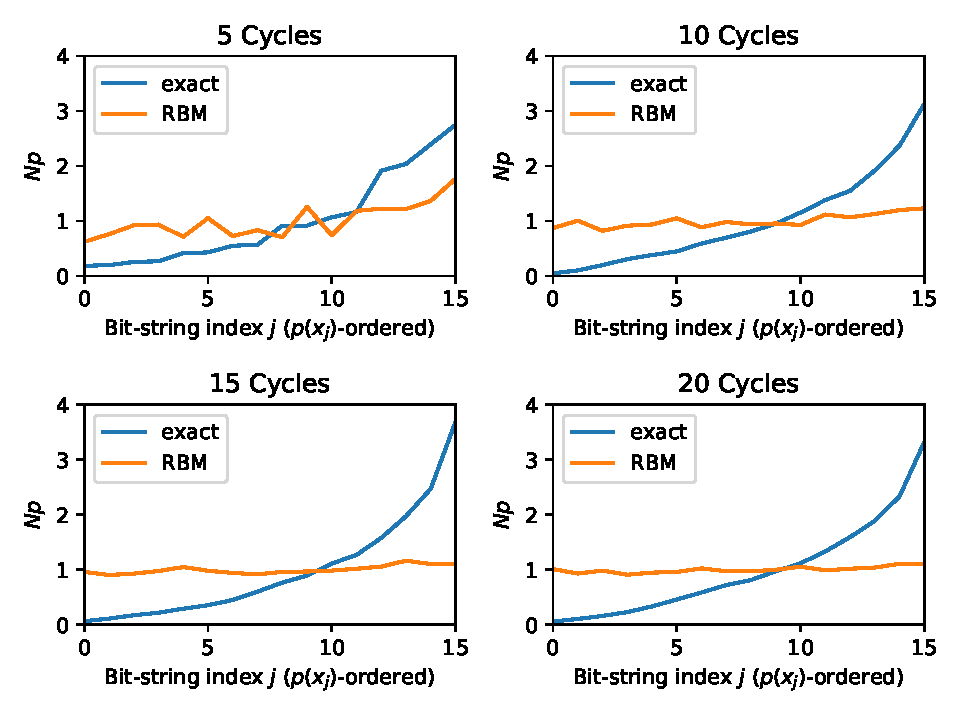
\includegraphics[width=\textwidth]{figures/results/AM-restarts-learned/avgPDF.pdf}
  \caption[Scaled average output probabilities of AdaMax with Restarts Learned]{
    Scaled average output probabilities of AdaMax with Restarts Learned. The true 
    output distribution approaches a Porter-Thomas shape with increasing number of cycles.}
  \label{fig:am_avgPDF}
\end{figure}

In figure~\ref{fig:am_avgBestPDF}, only the output distribution of the best performing RBMs with respect to the 
TVD are selected. Their outputs are averaged once again. The averaged best output distribution 
has a TVD of 0.00 for 5, 0.00 for 10, 0.00 for 15, and 0.00 for 20 
cycles. The cross entropy fidelity is 0.65 for 5, 0.72 for 10, 0.94 for 15 and 0.77 for 20 cycles each. 

\begin{figure}[H]
  \centering
  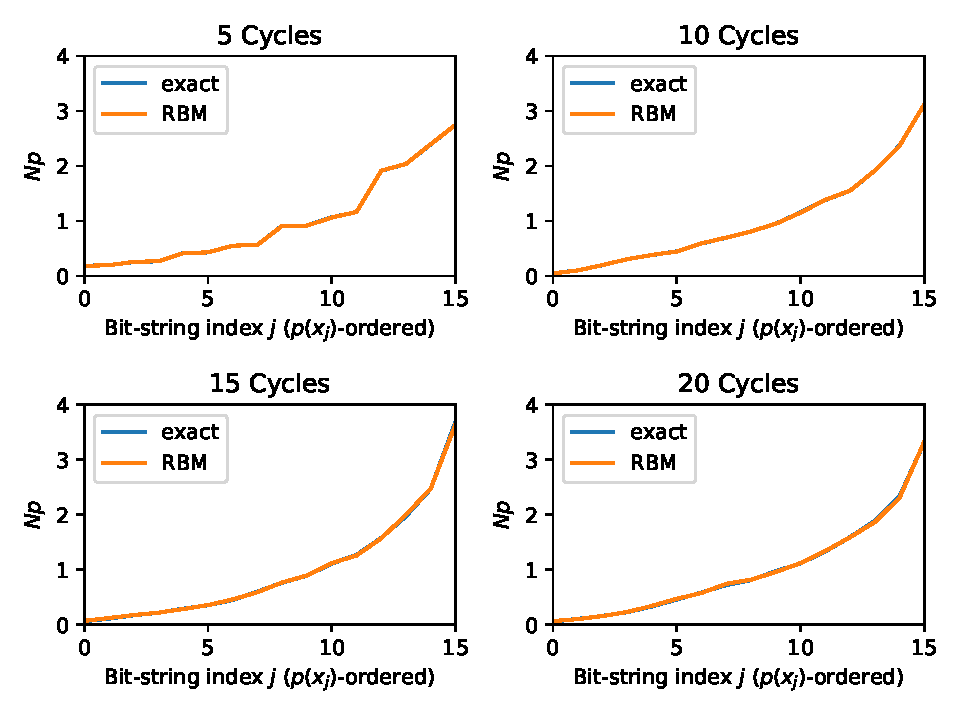
\includegraphics[width=\textwidth]{figures/results/AM-restarts-learned/avgBestPDF.pdf}
  \caption[Averaged best performing scaled output probabilities of AdaMax with Restarts Learned]{
    Scaled average output probabilities of AdaMax with Restarts Learned, only RBMs with lowest
    TVD for each circuit are considered. The true 
    output distribution approaches a Porter-Thomas shape with increasing number of cycles.}
  \label{fig:am_avgBestPDF}
\end{figure}

Figure~\ref{fig:am_tvd} and figure~\ref{fig:am_fxeb} give a more detailed overview of the influence of the 
number of training samples and training iterations on the TVD and cross entropy fidelity.

Except for the case of 8 samples, for AdaMax a higher number of training samples as well as a higher 
number of training iterations corresponds to a lower TVD. For 5 and 10 cycles, the TVD is lowest
when trained with 303 samples and 100,000 iterations. In these cases, it approaches 0.

For 15 and 20 cycles, the training process could not finish
within the given time frame with this combination of training parameters. On these circuits, the lowest TVDs have been achieved with 303 samples 
and 10,000 iterations.

Overall, the difference between 10,000 iterations and 100,0000 iterations is smaller than between 
1,000 iterations and 10,000 iterations. For 43 to 54 samples, the performance is similar in all cases.
Nevertheless, the TVD is lower with 54 samples than with 43 samples in all but one cases.

\begin{figure}[H]
  \centering
  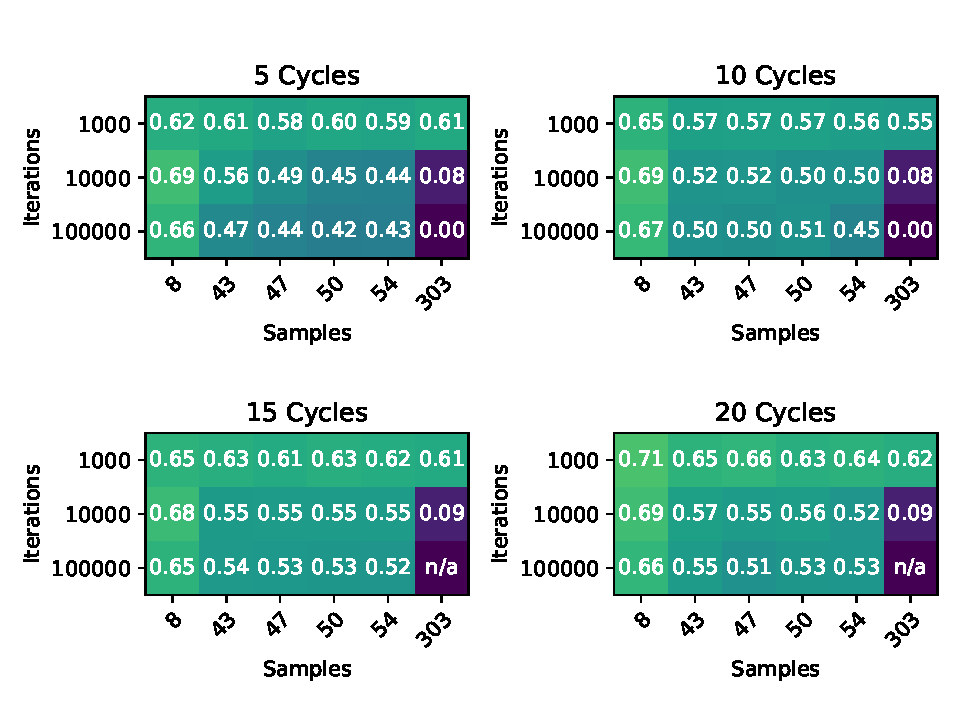
\includegraphics[width=\textwidth]{figures/results/AM-restarts-learned/tvd_heatmap.pdf}
  \caption[TVD of AdaMax with Restarts Learned]{TVD of Stochastic 
  Reconfiguration with Restarts Learned for the combinations of iterations and samples tested.
  For 100,000 iterations and 303 samples, the experiments did not finish within the time limit.}
  \label{fig:am_tvd}
\end{figure}

Figure~\ref{fig:am_fxeb} shows the average cross entropy fidelity achieved. In contrast to the case 
of TVD, a higher number of training samples and training iterations does not correlate with higher 
fidelities. Only in the case of 5 cycles, this correlation can be observed for 10,000 and 100,000 iterations.

The highest fidelities for 5 and 10 cycles are achieved for 303 samples and 100,000 iterations. For 
15 and 20 cycles, they are achieved with 303 samples and 10,000 iterations. 

In the case of 15 cycles, the overall highest fidelity of 0.90 had been measured. The highest fidelity is 0.65 for 5, 0.75 for 10, and 0.73 for 20 cycles.
This once again demonstrates that a lower TVD does not translate to a higher fidelity directly.

\begin{figure}[H]
  \centering
  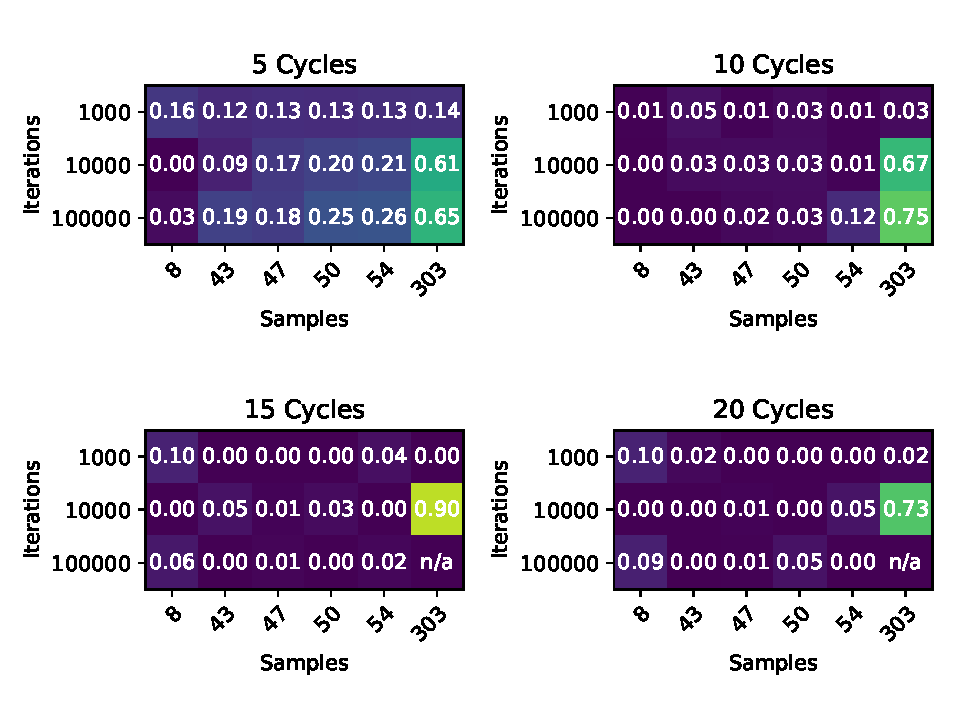
\includegraphics[width=\textwidth]{figures/results/AM-restarts-learned/fxeb_heatmap.pdf}
  \caption[Cross-entropy Fidelity of AdaMax with Restarts Learned]{Cross-entropy Fidelity of Stochastic 
  Reconfiguration with Restarts Learned for the combinations of iterations and samples tested.
  For 100,000 iterations and 303 samples, the experiments did not finish within the time limit.}
  \label{fig:am_fxeb}
\end{figure}

Figure~\ref{fig:am_overlap_8} to~\ref{fig:am_overlap_303} detail the mean log overlap of the RBMs during the 
training process when trained with 10,000 iterations for 8, 47, and 303 samples. The 
mean overlap of the RBM's state and the distribution implied by the training and test data sets are measured 
for each training iteration.
For 8 samples, the training and test overlaps don't vary much during the training process. The training errors on all three gates
close to 0 during the whole training process. The test error is at about 0.40 on the single-qubit gates. It is about 
0.9 on the $CZ$ gate.

\begin{figure}[H]
  \centering
  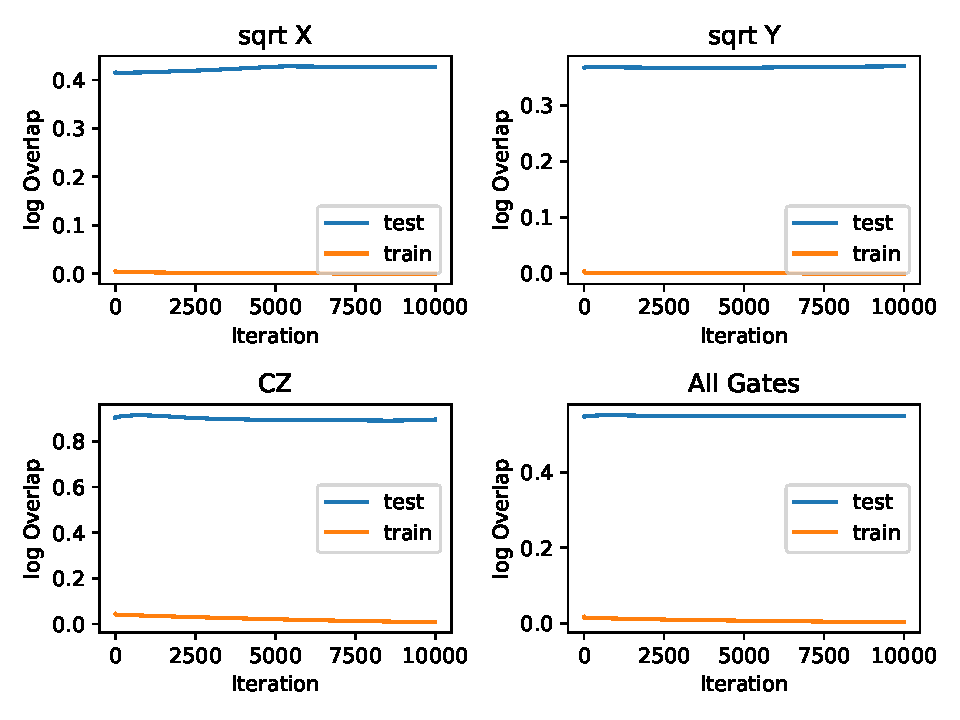
\includegraphics[width=\textwidth]{figures/results/AM-restarts-learned/avgOverlap_8.pdf}
  \caption[Training Overlap of AdaMax with Restarts Learned]{Training 
  Overlap of AdaMax with Restarts Learned for 8 samples.}
  \label{fig:am_overlap_8}
\end{figure}

For 47 samples, the log overlap on the training data drops almost to 0 within the first few iterations 
of training. There is only a small improvement to be observed in the $\sqrt{Y}$ gate afterward. 
The overlap on the test data drops to about 0.1 in the case of $\sqrt{X}$ gates within the first few iterations.
Afterward, there is a slight tendency upwards but the overlap stays in about that range. In the case 
of $\sqrt{Y}$ gates, the test overlap drops to about 0.11 within the first few iterations. Afterward, 
it slightly increases again before it reaches 0.11 after about 2,500 iterations again.

The log overlap looks different for the $CZ$ gate: After an initial drop of about 0.02 to 0.12, the 
training overlap slowly decreases until it reaches a value close to 0 . The 
training overlap takes a similar course. During the training process, it goes down to about 0.18, after 
starting at about 0.33.

The training and test overlap follow a similar course for 43, 50, and 54 samples. For 43 samples, the 
testing overlap reaches values slightly above 0.15 for the $\sqrt{X}$ and $\sqrt{Y}$ gate. On the $CZ$ gates, 
the overlap is only very slightly higher.

For 50 and 54 samples, the testing error goes down to about 0.075 for the $\sqrt{X}$ and $\sqrt{Y}$ gates. 
On the $CZ$ gates, the testing overlap goes down to about 0.15 over the course of the training. The graphs 
for 43, 50, and 54 qubits are included in the appendix.

\begin{figure}[H]
  \centering
  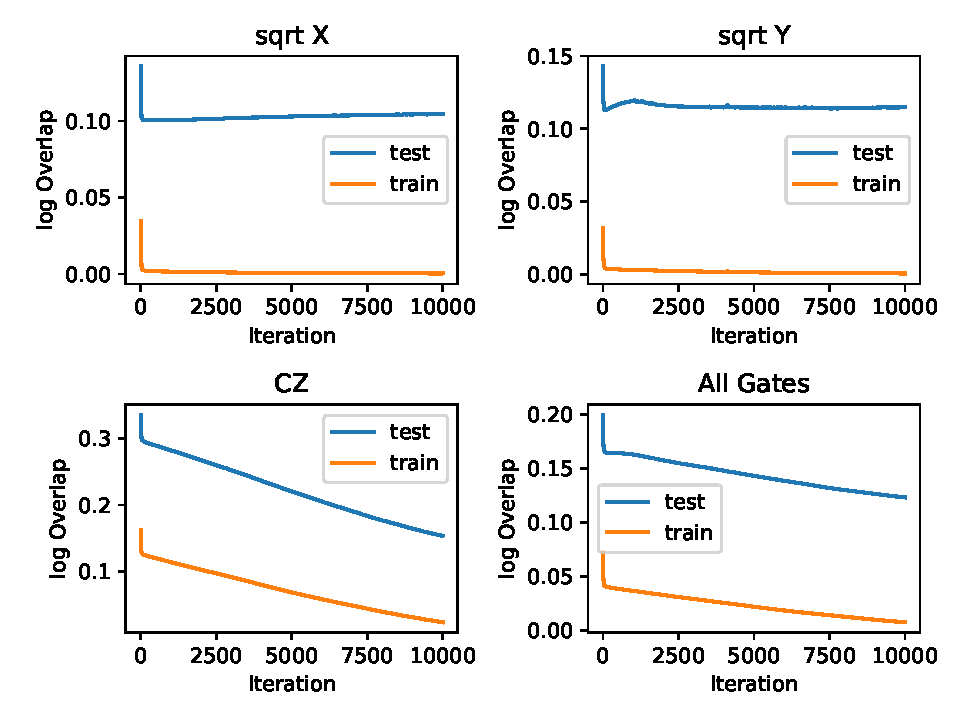
\includegraphics[width=\textwidth]{figures/results/AM-restarts-learned/avgOverlap_47.pdf}
  \caption[Training Overlap of AdaMax with Restarts Learned]{Training 
  Overlap of AdaMax with Restarts Learned for 47 samples.}
  \label{fig:am_overlap_47}
\end{figure}

For 303 training samples, the course of the training overlap is very similar to 47 samples.
A difference can be observed in the test overlap, which is very close to the training overlap 
throughout the whole training process.

\begin{figure}[H]
  \centering
  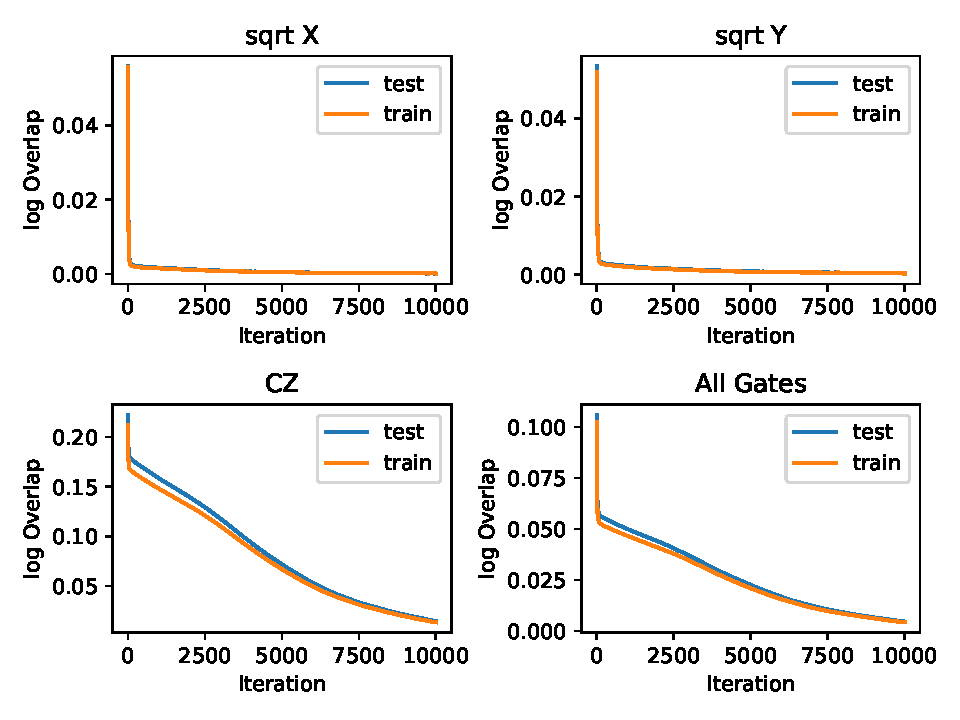
\includegraphics[width=\textwidth]{figures/results/AM-restarts-learned/avgOverlap_303.pdf}
  \caption[Training Overlap of AdaMax with Restarts Learned]{Training 
  Overlap of AdaMax with Restarts Learned for 303 samples.}
  \label{fig:am_overlap_303}
\end{figure}
